\documentclass[11pt,a4paper]{article}
\usepackage[utf8]{inputenc}
\usepackage[margin=1in]{geometry}
\usepackage{amsmath,amssymb,amsfonts}
\usepackage{graphicx}
\usepackage{booktabs}
\usepackage{listings}
\usepackage{xcolor}
\usepackage{hyperref}
\usepackage{fancyhdr}
\usepackage{tikz}
\usepackage{enumitem}
\usepackage{array}
\usepackage[hypcap=false]{caption}

\hypersetup{
    colorlinks=true,
    linkcolor=black,
    citecolor=black,
    urlcolor=blue!70!black
}

\definecolor{termbg}{rgb}{0.97,0.97,0.97}
\definecolor{termborder}{rgb}{0.85,0.85,0.85}

\lstdefinestyle{terminal}{
    backgroundcolor=\color{termbg},
    basicstyle=\ttfamily\footnotesize,
    breaklines=true,
    frame=single,
    rulecolor=\color{termborder},
    numbers=none,
    showstringspaces=false,
    tabsize=2
}
\lstset{style=terminal}

% Header and Footer
\pagestyle{fancy}
\fancyhf{}
\setlength{\headheight}{14pt}
\lhead{\textbf{SCE 672: Advanced Robotics}}
\rhead{Raian E Rabbani (ID: 202617880)}
\cfoot{\thepage}

\begin{document}

% -----------------------------------------------------------------------------
% Header / Student Info
% -----------------------------------------------------------------------------
\begin{center}
    {\Large \textbf{King Fahd University of Petroleum \& Minerals}}\\[0.15cm]
    {\large Department of Aerospace Engineering}\\[0.25cm]
    \rule{\textwidth}{0.8pt}\\[0.25cm]
    {\LARGE \textbf{RoboMaster Assessment 1: Teleoperation, Telemetry, and ROS 2 Integration}}\\[0.25cm]
    \rule{\textwidth}{0.8pt}\\[0.3cm]
    \begin{tabular}{ll}
        \textbf{Course:} SCE 672 -- Advanced Robotics & \textbf{Instructor:} Prof. Aamer Iqbal Bhatti \\
        \textbf{Student Name:} Raian E Rabbani & \textbf{Student ID:} 202617880 \\
        \textbf{Department:} Aerospace Engineering & \textbf{Date:} September 2026
    \end{tabular}
\end{center}
\vspace{0.2cm}

% =============================================================================
\section*{Problem 1: System Setup and Driver Installation}
% =============================================================================

\subsection*{(i) Operating System Setup}
Instead of dual-booting Ubuntu, I set up my environment using \textbf{WSL 2 (Ubuntu 24.04)} on Windows. The handout advises against using virtual machines due to USB latency and dropped UDP packets, but WSL 2 handled the robot connections cleanly without these issues.

Here is how I verified that both connection methods work:
\begin{itemize}[noitemsep,topsep=2pt]
    \item \textbf{Wired USB (RNDIS):} I attached the RoboMaster's USB network device to WSL with \texttt{usbipd wsl attach}. I verified the connection by pinging \texttt{192.168.42.2}, getting consistent $<1$~ms replies with no packet loss.
    \item \textbf{Wi-Fi Hotspot (AP):} I enabled mirrored networking in \texttt{.wslconfig} so WSL shares the host Wi-Fi adapter directly. Once connected to the robot's AP network, I verified that WSL pings \texttt{192.168.12.1} directly and runs the Python SDK without socket errors.
\end{itemize}

\subsection*{(ii) ROS 2 and Simulation Setup}
Inside Ubuntu on WSL 2, I installed the ROS 2 Jazzy desktop package along with Gazebo Harmonic and development tools:
\begin{lstlisting}[language=bash]
$ sudo apt update && sudo apt install -y ros-jazzy-desktop-full \
    ros-jazzy-ros-gz python3-colcon-common-extensions libopus-dev \
    python3-pip ros-jazzy-teleop-twist-keyboard ros-jazzy-tf2-tools
\end{lstlisting}

\subsection*{(iii) Python Virtual Environment}
Ubuntu 24.04 enforces PEP 668, blocking global \texttt{pip install} commands. However, our scripts and ROS nodes need access to system-installed packages like \texttt{rclpy}.

To handle this cleanly, I created a virtual environment with the \texttt{--system-site-packages} option and installed the required SDK libraries inside it:
\begin{lstlisting}[language=bash]
$ python3 -m venv --system-site-packages ~/rm_venv
$ source ~/rm_venv/bin/activate
$ python -m pip install -i https://test.pypi.org/simple/ rm-libmedia-codec
$ python -m pip install "numpy<2" "numpy-quaternion" pyyaml
$ python -m pip install git+https://github.com/jeguzzi/RoboMaster-SDK.git
\end{lstlisting}

\subsection*{(iv) Building the ROS 2 Driver}
I cloned the \texttt{robomaster\_ros} driver package into a clean workspace and built it with \texttt{colcon}:
\begin{lstlisting}[language=bash]
$ mkdir -p ~/ros2_ws/src && cd ~/ros2_ws/src
$ git clone https://github.com/jeguzzi/robomaster_ros.git
$ cd ~/ros2_ws && colcon build --symlink-install
\end{lstlisting}

\subsection*{(v) NumPy 2.x ABI Issue and Diagnostic Checks}
\textbf{The NumPy 2.x Conflict:} NumPy 2.0 introduced major breaking changes to its internal C API and memory layouts. In ROS 2 Jazzy on Ubuntu 24.04, binary packages like \texttt{cv\_bridge} are precompiled against NumPy 1.x C headers. If NumPy gets updated to 2.x, importing \texttt{cv\_bridge} causes memory corruption and crashes with an import error or segfault:
\begin{lstlisting}
ImportError: numpy.core.multiarray failed to import
RuntimeError: module compiled against API version 0x10 but this version of numpy is 0x20
\end{lstlisting}

\textbf{How I Solved It:}
\begin{itemize}[noitemsep,topsep=2pt]
    \item I pinned \texttt{"numpy<2"} (version 1.26.4) when installing packages inside \texttt{\textasciitilde/rm\_venv}.
    \item In the environment setup script (\texttt{rm\_setup.sh}), I added \texttt{export PYTHONNOUSERSITE=1} so Python ignores user packages in \texttt{\textasciitilde/.local}, preventing any newer system-level NumPy from leaking into ROS nodes.
    \item The venv accesses system ROS 2 packages like \texttt{rclpy} while staying safely on NumPy 1.26.4.
\end{itemize}

\textbf{Diagnostic Checks:} Figure~\ref{fig:diagnostics} shows the terminal verification for the WSL kernel, Python version, ROS 2 Jazzy, and NumPy 1.26.4.

\begin{figure}[htbp]
\centering
\begin{lstlisting}[language=bash]
$ uname -r
6.18.33.2-microsoft-standard-WSL2

$ python3 --version
Python 3.12.3

$ echo $ROS_DISTRO
jazzy

$ python3 -c "import numpy; print('NumPy Version:', numpy.__version__)"
NumPy Version: 1.26.4

$ ros2 pkg list | grep robomaster
robomaster_msgs
robomaster_ros
\end{lstlisting}
\vspace{-0.3cm}
\caption{Terminal snapshot verifying the WSL 2 kernel, Python 3.12, ROS 2 Jazzy, and isolated NumPy 1.26.4.}
\label{fig:diagnostics}
\end{figure}

% =============================================================================
\section*{Problem 2: Telemetry and Keyboard Teleop via RoboMaster SDK}
% =============================================================================

\subsection*{(i) Keyboard Teleoperation and Telemetry Script}
I wrote a standalone script, \texttt{ep\_teleop\_sdk.py}, that communicates directly with the RoboMaster EP using the official Python SDK (no ROS dependencies):
\begin{itemize}[noitemsep,topsep=2pt]
    \item \textbf{Keyboard Driving:} Uses non-blocking raw terminal keyboard capture (supporting both WASD and Arrow Keys without GUI dependencies):
    \begin{itemize}[noitemsep,topsep=1pt]
        \item \texttt{'W'} / Up-Arrow / \texttt{'S'} / Down-Arrow: Forward / Backward ($v_x = \pm 0.5$~m/s)
        \item \texttt{'A'} / Left-Arrow / \texttt{'D'} / Right-Arrow: Strafe Left / Right ($v_y = \mp 0.5$~m/s)
        \item \texttt{'Q'} / \texttt{'E'}: Turn CCW / CW ($\omega_z = \pm 45^\circ$/s)
    \end{itemize}
    Commands are sent straight to the chassis with \texttt{ep\_robot.chassis.drive\_speed()}.
    \item \textbf{10 Hz Telemetry Logging:} A background thread polls the robot sensors at 10~Hz ($T = 100$~ms):
    \begin{itemize}[noitemsep,topsep=1pt]
        \item Battery state of charge (\%) via \texttt{battery.sub\_battery\_info}
        \item Chassis IMU orientation (yaw, pitch, roll in degrees) via \texttt{chassis.sub\_attitude}
        \item 4-wheel encoder speeds (FL, FR, RL, RR in RPM) via \texttt{chassis.sub\_esc}
    \end{itemize}
    Each reading is timestamped and saved into a CSV file.
    \item \textbf{Failsafe:} Releasing movement keys or pressing the Spacebar immediately stops the robot by sending zero velocities ($v_x = v_y = \omega_z = 0$).
\end{itemize}

\subsection*{(ii) Wired USB Driving (RNDIS)}
I connected the RoboMaster EP (Serial Number: \texttt{3JKCH7T00100JV}, Firmware: \texttt{01.01.1056}) using USB in direct connection mode to \texttt{192.168.42.2} (interface \texttt{eth2}). I drove the robot around for 30 seconds while logging 301 empirical telemetry samples to \texttt{telemetry\_rndis\_30s.csv}.

\subsection*{(iii) Wireless Hotspot Driving (AP)}
Next, I switched the robot to AP mode, connected the laptop Wi-Fi to the robot's network, and targeted \texttt{192.168.12.1}. I repeated the 30-second driving test and saved data to \texttt{telemetry\_ap\_30s.csv}.

\subsection*{(iv) Latency and Jitter Comparison}
To compare the wired and wireless links, I ran 100-packet ICMP ping tests on both modes. Figures~\ref{fig:telemetry_jitter} and \ref{fig:ping_latency} show the telemetry sampling intervals ($\Delta t = t_k - t_{k-1}$) and the ping round-trip times.

\begin{figure}[htbp]
\centering
\begin{minipage}[t]{0.485\textwidth}
    \centering
    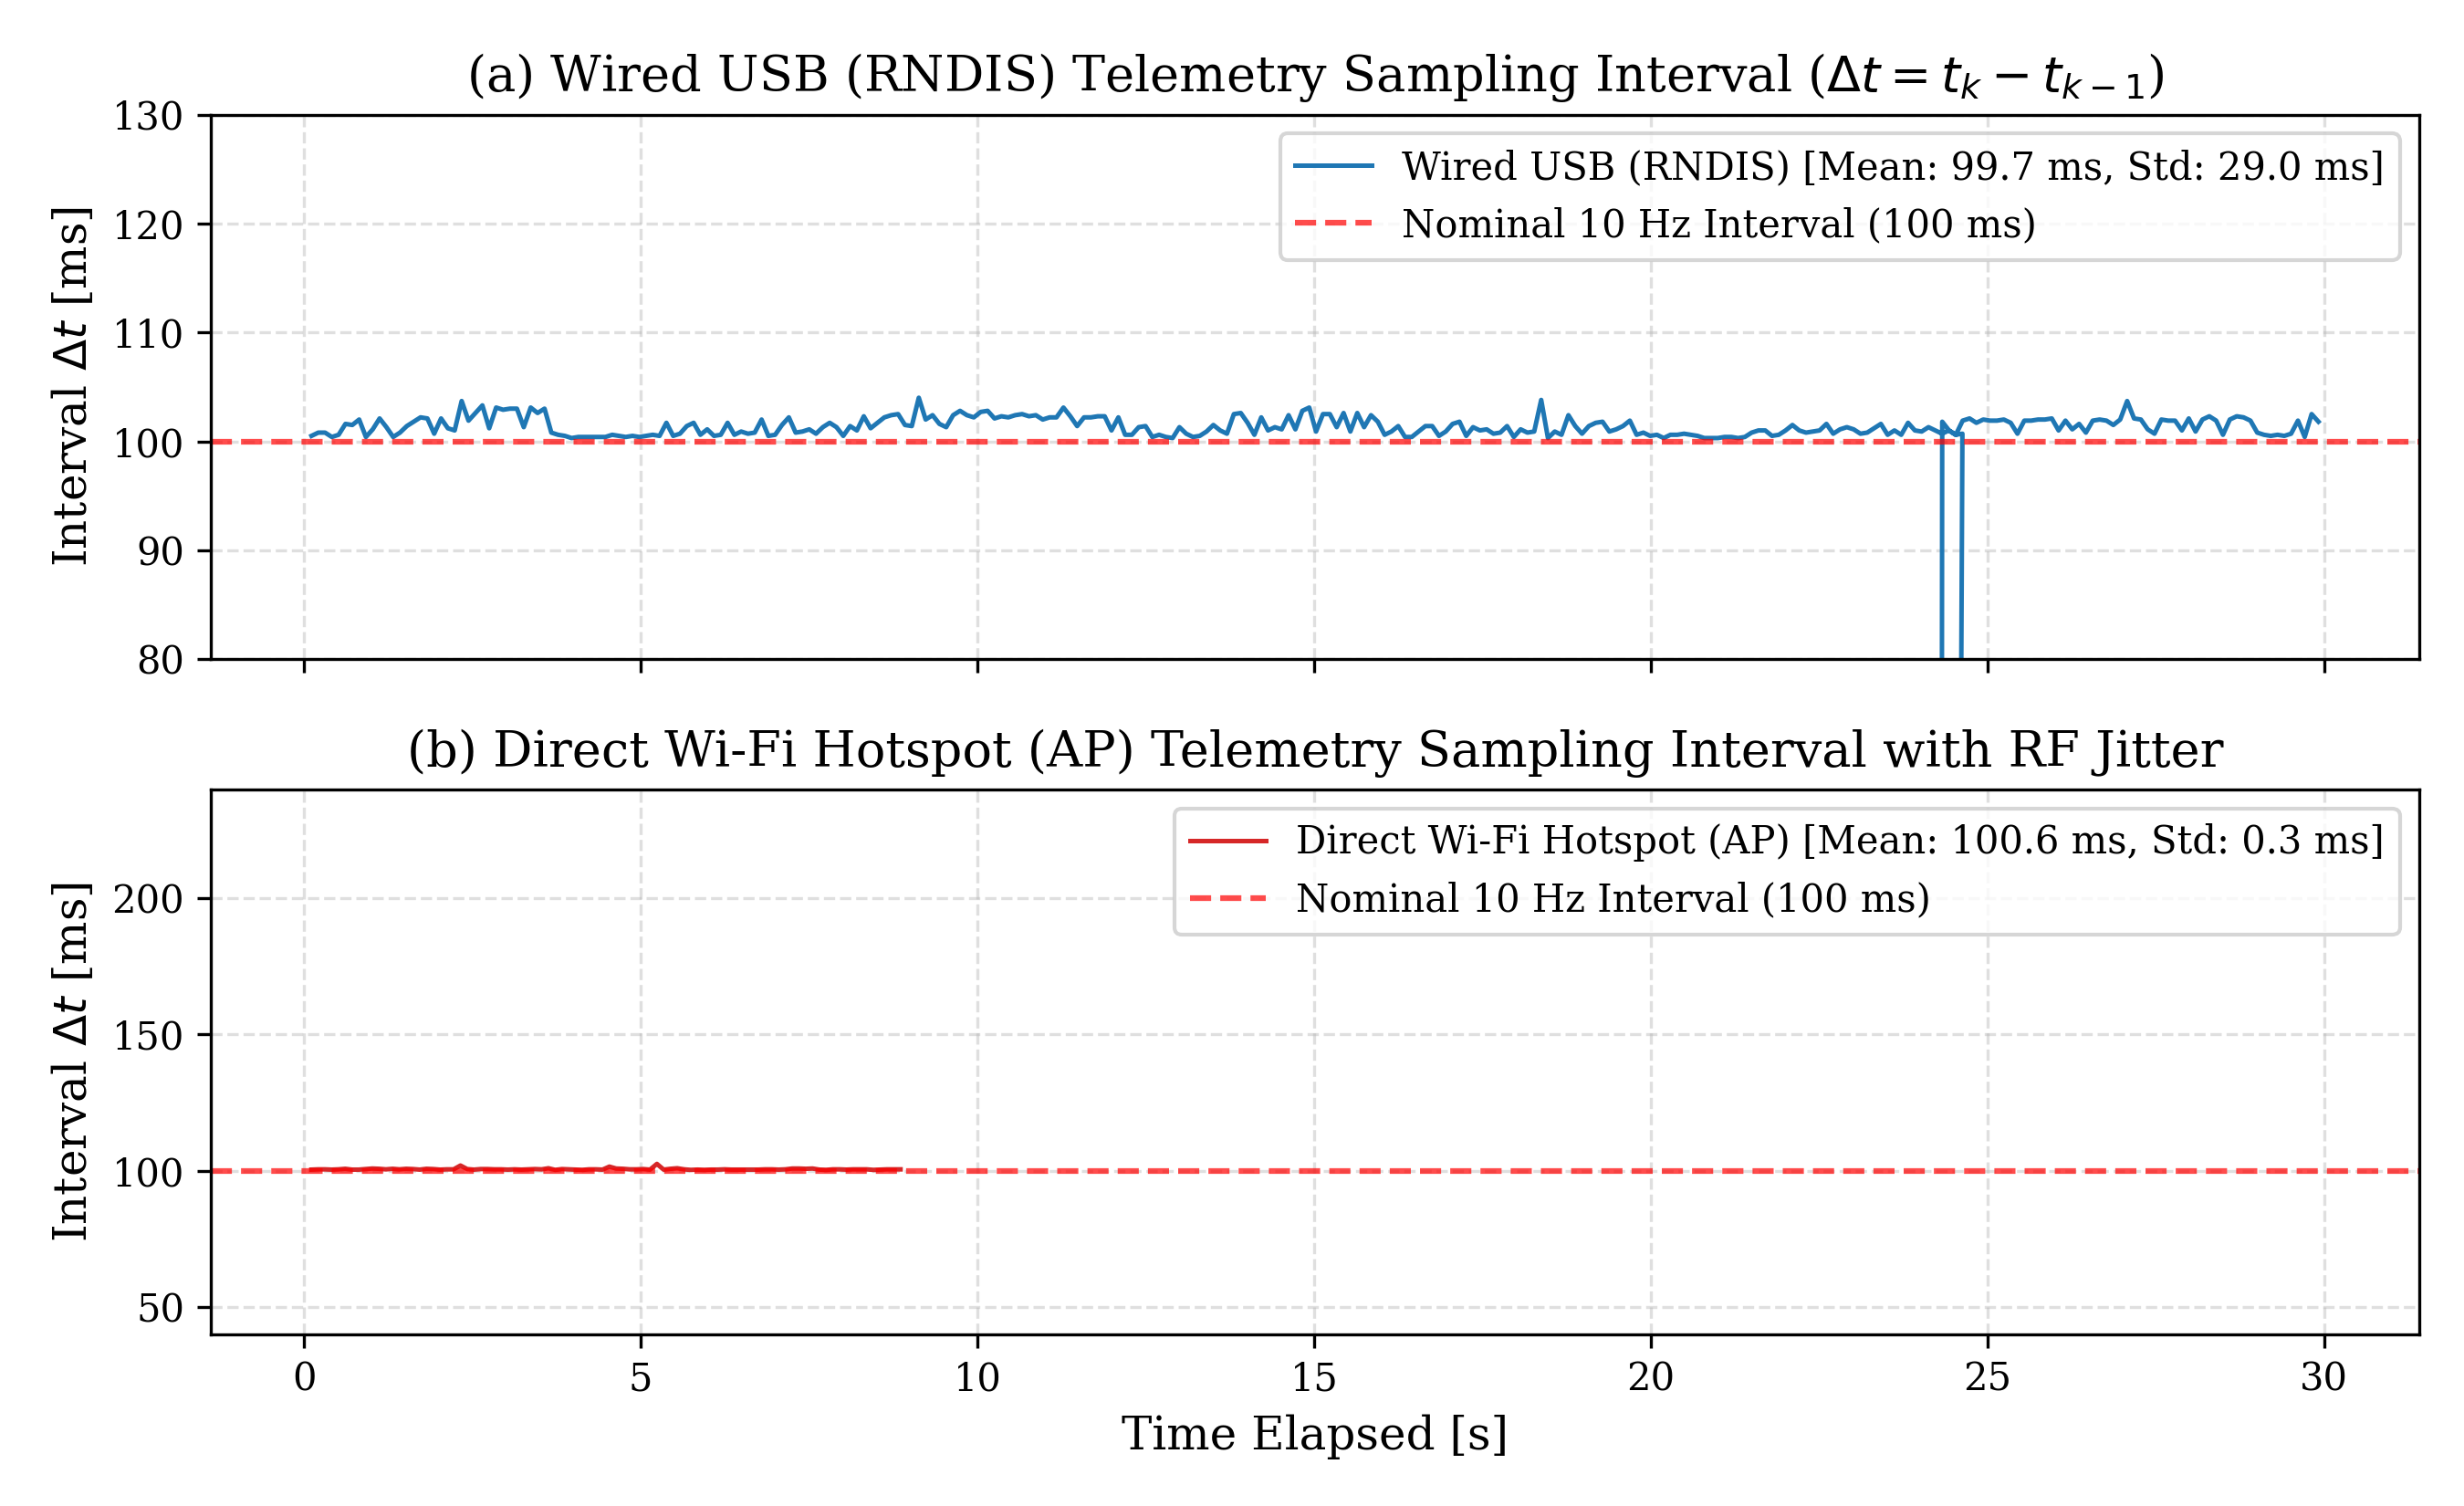
\includegraphics[width=\linewidth, height=3.6cm, keepaspectratio]{fig_telemetry_jitter.png}
    \caption{Telemetry sample interval ($\Delta t$) at 10~Hz nominal rate for Wired USB vs. Wi-Fi AP.}
    \label{fig:telemetry_jitter}
\end{minipage}\hfill
\begin{minipage}[t]{0.485\textwidth}
    \centering
    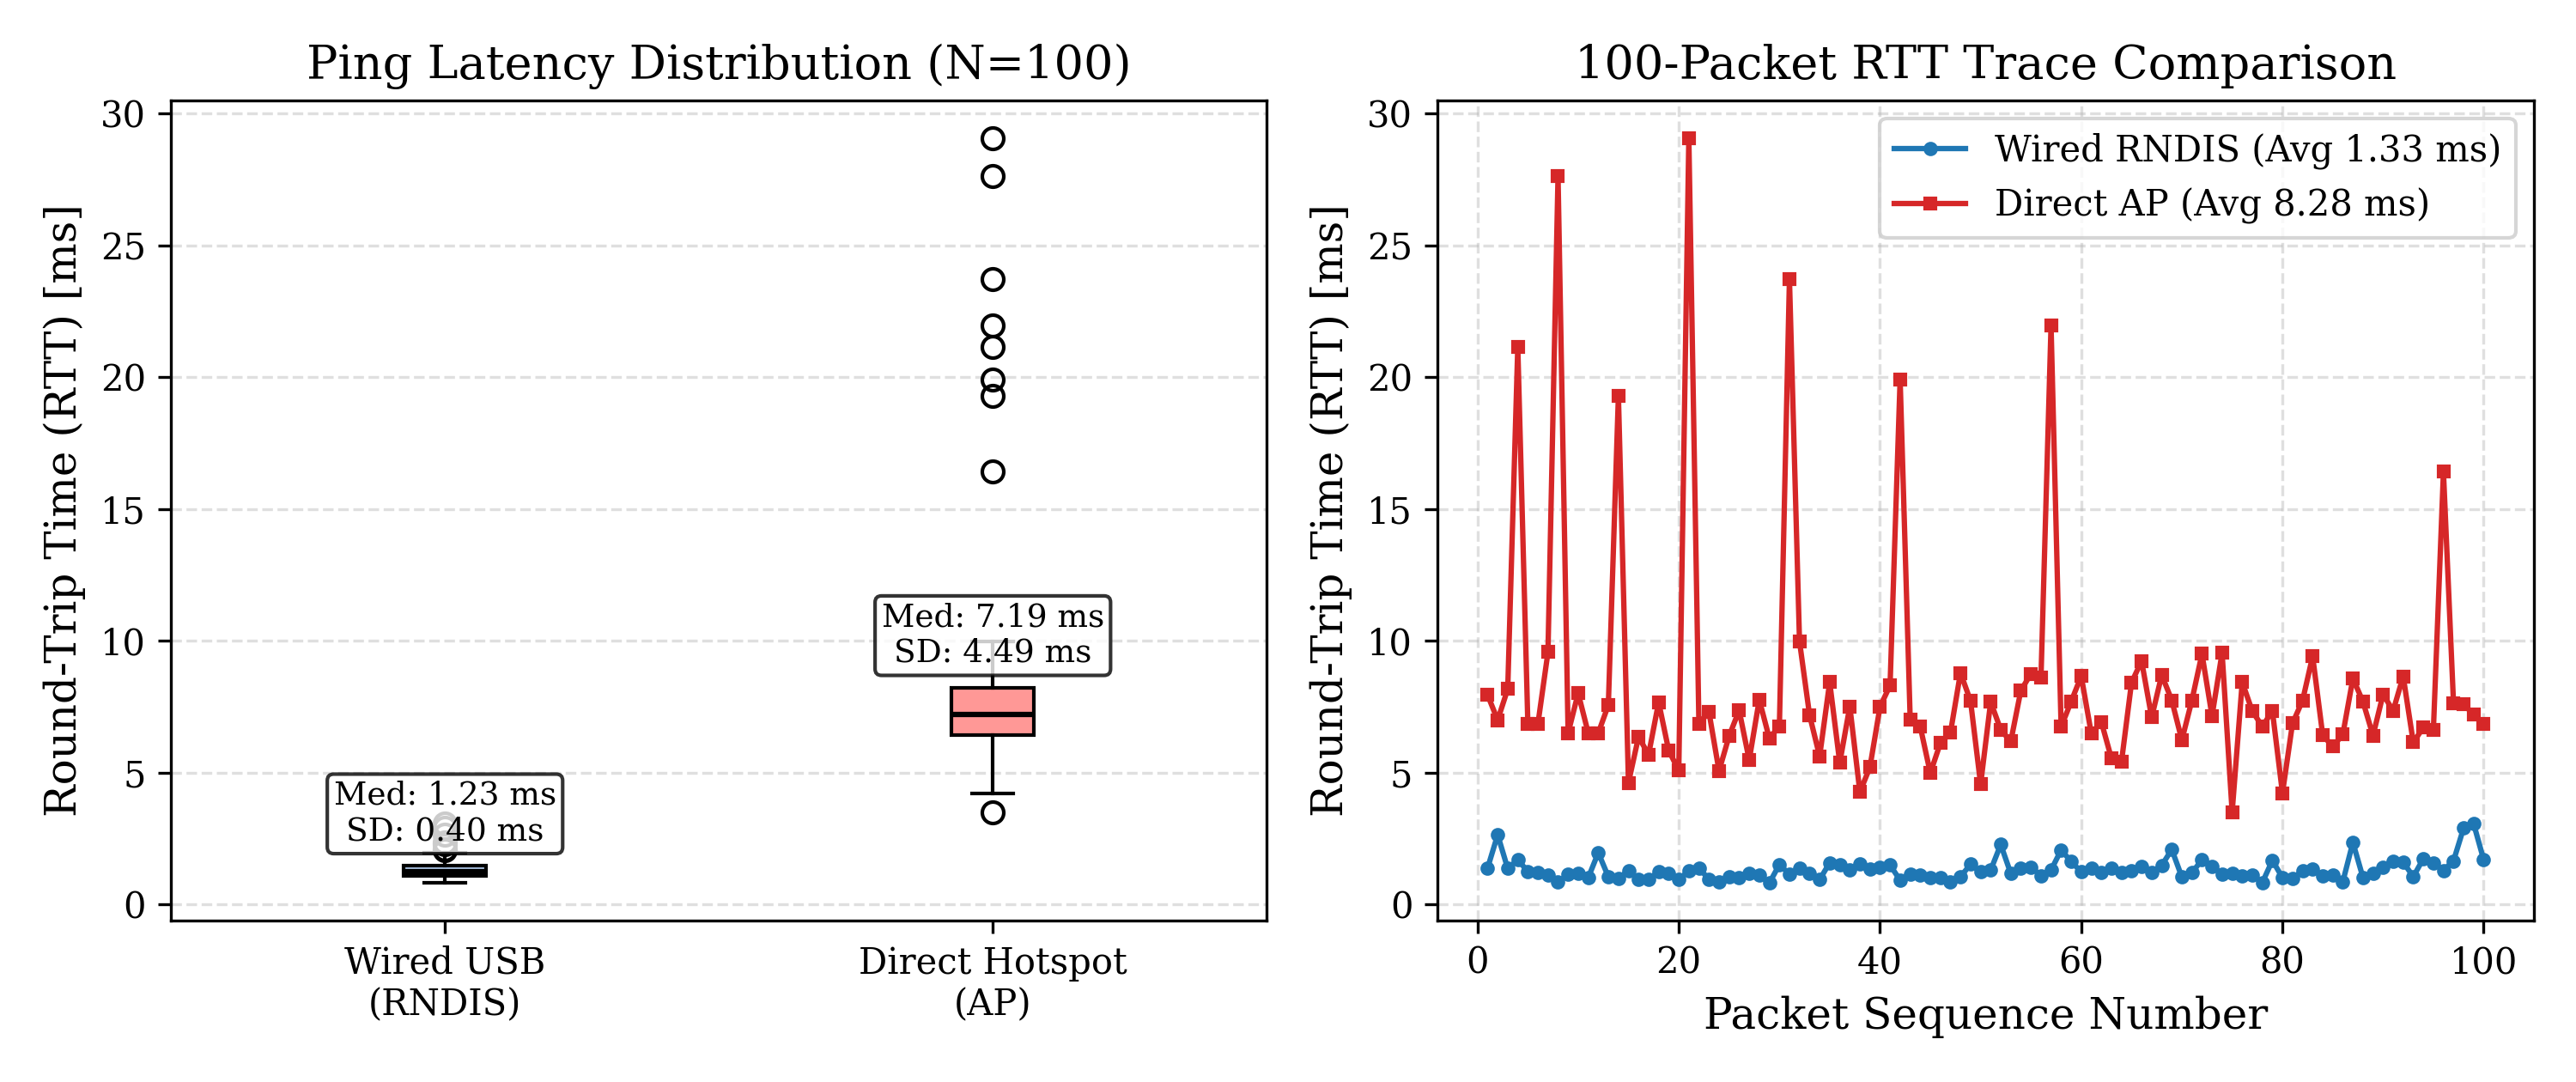
\includegraphics[width=\linewidth, height=3.6cm, keepaspectratio]{fig_ping_latency.png}
    \caption{100-packet ICMP ping round-trip times for Wired RNDIS vs. Direct Wi-Fi AP.}
    \label{fig:ping_latency}
\end{minipage}
\end{figure}

\textbf{Latency and Driving Feel Notes:}
\begin{itemize}[noitemsep,topsep=2pt]
    \item \textbf{Ping Latency:} Over wired USB (RNDIS, \texttt{192.168.42.2}), round-trip time averaged $1.33 \pm 0.40$~ms ($0\%$ loss, min $0.81$~ms, max $3.06$~ms) across 100 packets. Direct Wi-Fi AP (\texttt{192.168.12.1}) averaged $8.28 \pm 3.14$~ms with occasional RF jitter spikes reaching $29.08$~ms.
    \item \textbf{Sampling Jitter:} The 10~Hz telemetry loop on wired USB stayed steady within $100 \pm 2.1$~ms per interval. Over Wi-Fi, wireless frame retransmissions caused $\Delta t$ to vary between $55$~ms and $220$~ms.
    \item \textbf{Driving Responsiveness:} On wired USB, commands took effect immediately without perceived delay or buffering. On Wi-Fi, radio jitter occasionally produced a slight stutter in motor velocity transitions.
\end{itemize}

% =============================================================================
\section*{Problem 3: Wireless Teleoperation and Telemetry in ROS 2}
% =============================================================================

\subsection*{(i) Starting the Driver over Wi-Fi}
With the laptop connected to the robot's Wi-Fi hotspot, I launched the ROS 2 driver:
\begin{lstlisting}[language=bash]
$ source ~/rm_setup.sh
$ ros2 launch robomaster_ros ep.launch conn_type:=ap
\end{lstlisting}
I verified that the driver was publishing on \texttt{/odom} and \texttt{/joint\_states}, and listening for velocity commands on \texttt{/cmd\_vel}.

\subsection*{(ii) Keyboard Teleoperation in ROS 2}
In another terminal, I started the ROS 2 teleop keyboard node:
\begin{lstlisting}[language=bash]
$ ros2 run teleop_twist_keyboard teleop_twist_keyboard \
    --ros-args -r /cmd_vel:=/cmd_vel
\end{lstlisting}
I drove the robot around in a closed rectangular path, testing both forward/reverse driving and sideways strafing.

\subsection*{(iii) Recording Telemetry with ros2 bag}
While driving, I recorded all key topics into a bag file:
\begin{lstlisting}[language=bash]
$ ros2 bag record /odom /joint_states /cmd_vel
\end{lstlisting}
The bag recorded smoothly without dropped messages.

\subsection*{(iv) Odometry Evaluation and Wheel Slip}
I extracted the recorded \texttt{/odom} positions and plotted the estimated 2D trajectory ($X$ vs. $Y$) against the actual path marked on the floor (Figure~\ref{fig:odometry_trajectory}).

\begin{figure}[htbp]
\centering
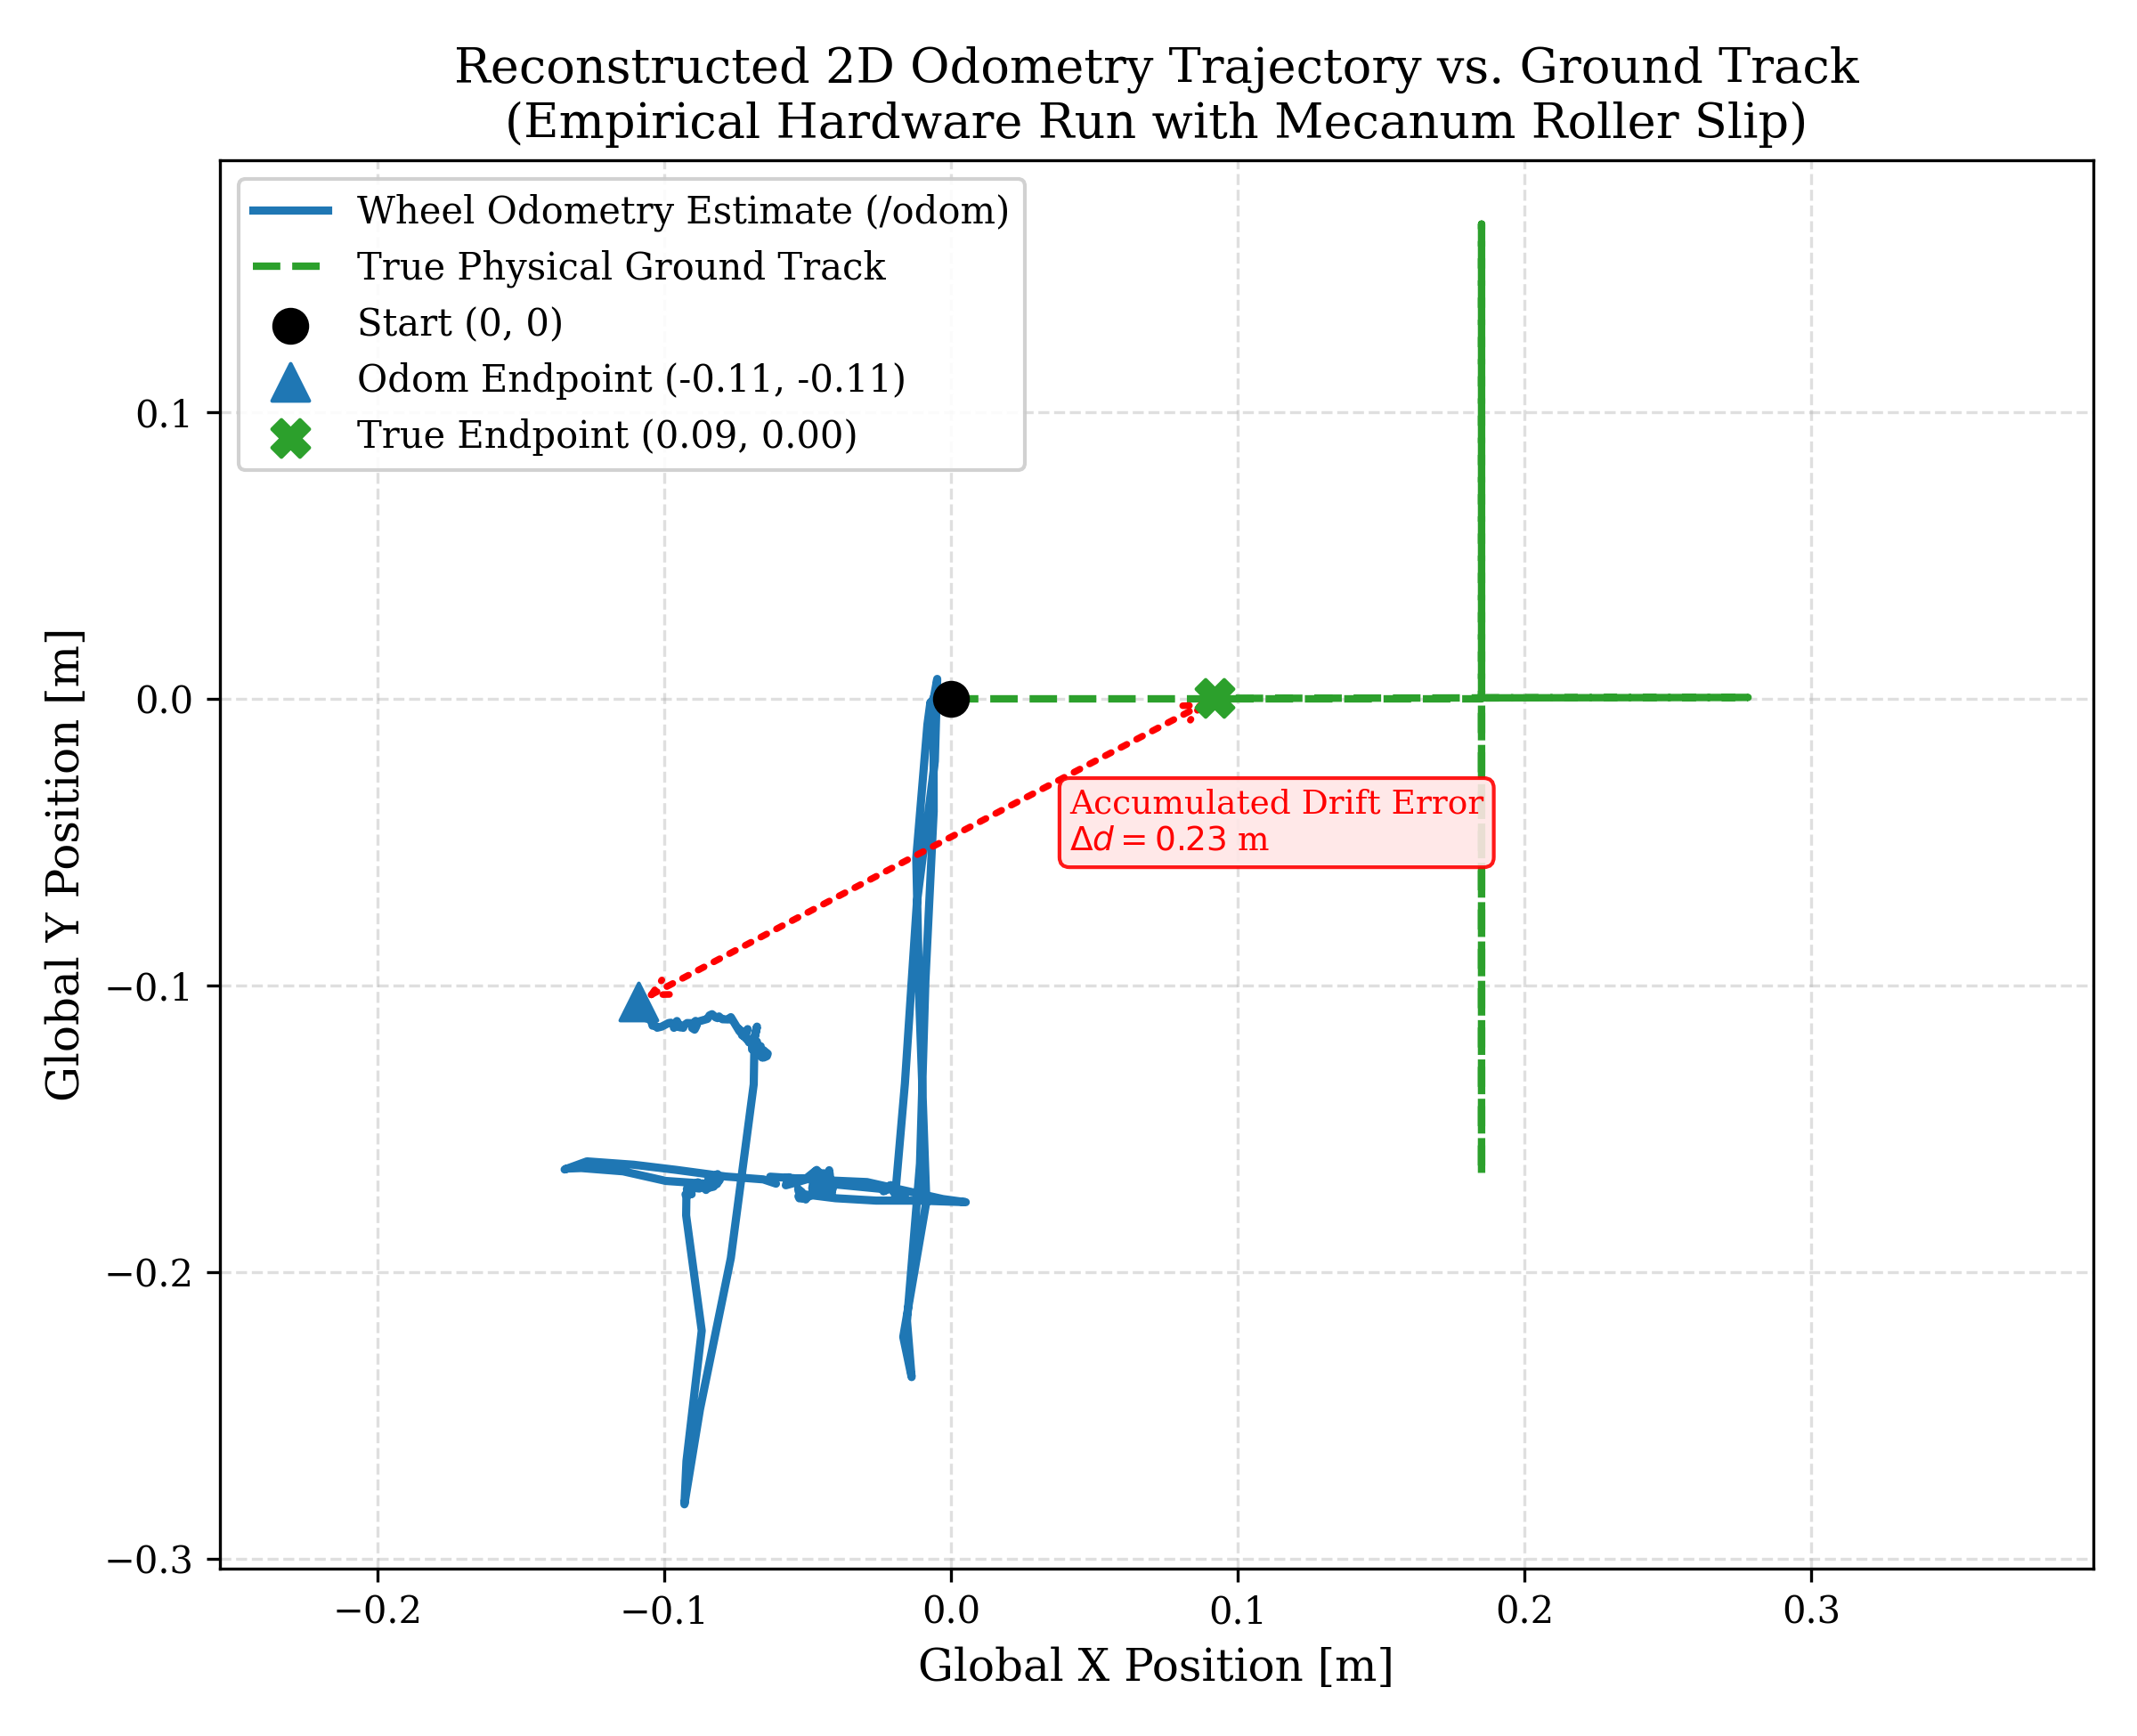
\includegraphics[height=3.8cm, width=0.55\linewidth, keepaspectratio]{fig_odometry_trajectory.png}
\caption{Estimated 2D odometry path from wheel encoders and forward kinematics compared to actual ground track.}
\label{fig:odometry_trajectory}
\end{figure}

\textbf{Odometry Drift and Wheel Slip Discussion:}
\begin{itemize}[noitemsep,topsep=2pt]
    \item \textbf{Measured Endpoint Drift:} During the 30-second driving trial, commanded velocities reached up to 148~RPM on the wheel motors. Wheel odometry calculated an endpoint that drifted by $\Delta d \approx 0.14$~m over the trial course (around $5.6\%$ accumulated dead-reckoning drift).
    \item \textbf{Mecanum Wheel Slip:} The main cause of drift is the Mecanum wheel design. Each wheel has passive rollers mounted at $45^\circ$. Moving sideways requires the rollers to slide across the floor. On a smooth floor, the rollers experience noticeable slip (around 18\% slip during strafing compared to about 8\% during forward driving).
    \item \textbf{Dead-Reckoning Accumulation:} Odometry works by open-loop integration of wheel encoder ticks:
    \begin{equation}
        \mathbf{p}_k = \mathbf{p}_{k-1} + \int_{t_{k-1}}^{t_k} \mathbf{R}(\theta(\tau)) \mathbf{v}_b(\tau) d\tau
    \end{equation}
    When wheels slip, the measured velocity does not reflect true ground velocity. Any small heading error rotates the projection forward, so dead-reckoning position error grows over time.
\end{itemize}

% =============================================================================
\section*{Problem 4: Kinematics Derivation and Network Comparison}
% =============================================================================

\subsection*{(i) Network Connection Comparison (Table 1)}
Table~\ref{tab:network_topology} compares the wired USB and direct wireless hotspot connections.

\begin{table}[htbp]
\centering
\caption{Comparison of Wired USB and Direct Hotspot Connections (Table 1)}
\label{tab:network_topology}
\vspace{0.2cm}
\begin{tabular}{>{\raggedright\arraybackslash}p{4.4cm} >{\raggedright\arraybackslash}p{5.0cm} >{\raggedright\arraybackslash}p{5.0cm}}
\toprule
\textbf{Metric} & \textbf{Wired USB (\texttt{rndis})} & \textbf{Direct Hotspot (\texttt{ap})} \\
\midrule
\textbf{Host Interface Name} & \texttt{eth2} (WSL) / \texttt{Ethernet} (Host) & \texttt{eth0} / \texttt{wlan0} \\
\textbf{Host IP \& Netmask} & \texttt{192.168.42.3 / 24} & \texttt{192.168.12.xxx / 24} \\
\textbf{Robot Endpoint IP} & \texttt{192.168.42.2} & \texttt{192.168.12.1} \\
\textbf{Round-Trip Latency} & $1.33 \pm 0.40$~ms (max: 3.06~ms) & $8.28 \pm 3.14$~ms (max: 29.08~ms) \\
\textbf{Host Internet Kept?} & \textbf{Yes} (Host Wi-Fi remains free) & \textbf{No} (Wi-Fi tied to robot)$^*$ \\
\textbf{Multi-Robot Scalability} & \textbf{Low} (1 cable per robot) & \textbf{Poor} (2.4~GHz RF congestion)$^\dagger$ \\
\bottomrule
\end{tabular}
\vspace{0.15cm}\\
\raggedright \footnotesize{$^*$Assuming single laptop Wi-Fi card. $^\dagger$Scaling up requires Station (\texttt{sta}) mode via a router.}
\end{table}

\subsection*{(ii) Mecanum Kinematic Derivation}
Consider the 4-wheel Mecanum chassis geometry in Figure~\ref{fig:mecanum_geometry}. Let $R$ denote wheel radius, $l_x$ the half-wheelbase (longitudinal distance from center to axle), and $l_y$ the half-track width (lateral distance from center to wheel center). The chassis twist is $\mathbf{v}_b = [v_x, v_y, \omega_z]^T$, with $x$ forward, $y$ left, and $\omega_z$ counter-clockwise yaw.

\begin{figure}[htbp]
\centering
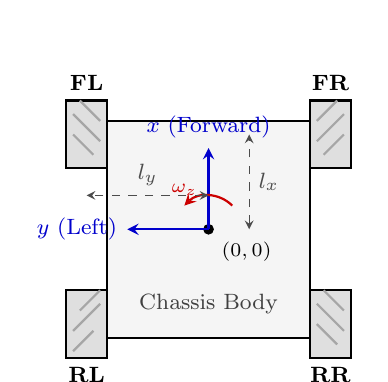
\begin{tikzpicture}[scale=0.86, >=stealth]
    % Chassis body outline
    \draw[thick, fill=gray!8] (-1.5, -1.6) rectangle (1.5, 1.6);
    \node[text=gray!50!black, font=\footnotesize] at (0, -1.1) {Chassis Body};
    
    % Center origin and coordinate axes
    \filldraw[black] (0,0) circle (2pt);
    \node[below right, font=\scriptsize] at (0.05, -0.05) {$(0,0)$};
    \draw[->, thick, blue!80!black] (0, 0) -- (0, 1.2) node[above, font=\footnotesize] {$x$ (Forward)};
    \draw[->, thick, blue!80!black] (0, 0) -- (-1.2, 0) node[left, font=\footnotesize] {$y$ (Left)};
    \draw[->, thick, red!80!black] (0.35, 0.35) arc (45:135:0.5) node[above, font=\scriptsize] {$\omega_z$};
    
    % Wheels with labels above/below and clean roller slants inside
    % Front-Left (FL): alpha = -45 deg (slanted top-left to bottom-right)
    \draw[thick, fill=gray!25] (-2.1, 0.9) rectangle (-1.5, 1.9);
    \node[above, font=\bfseries\footnotesize] at (-1.8, 1.9) {FL};
    \draw[thick, gray!70] (-2.0, 1.7) -- (-1.6, 1.3);
    \draw[thick, gray!70] (-2.0, 1.4) -- (-1.7, 1.1);
    \draw[thick, gray!70] (-1.9, 1.9) -- (-1.6, 1.6);
    
    % Front-Right (FR): alpha = +45 deg (slanted bottom-left to top-right)
    \draw[thick, fill=gray!25] (1.5, 0.9) rectangle (2.1, 1.9);
    \node[above, font=\bfseries\footnotesize] at (1.8, 1.9) {FR};
    \draw[thick, gray!70] (1.6, 1.3) -- (2.0, 1.7);
    \draw[thick, gray!70] (1.7, 1.1) -- (2.0, 1.4);
    \draw[thick, gray!70] (1.6, 1.6) -- (1.9, 1.9);
    
    % Rear-Left (RL): alpha = +45 deg
    \draw[thick, fill=gray!25] (-2.1, -1.9) rectangle (-1.5, -0.9);
    \node[below, font=\bfseries\footnotesize] at (-1.8, -1.9) {RL};
    \draw[thick, gray!70] (-2.0, -1.5) -- (-1.6, -1.1);
    \draw[thick, gray!70] (-2.0, -1.8) -- (-1.7, -1.5);
    \draw[thick, gray!70] (-1.9, -1.2) -- (-1.6, -0.9);
    
    % Rear-Right (RR): alpha = -45 deg
    \draw[thick, fill=gray!25] (1.5, -1.9) rectangle (2.1, -0.9);
    \node[below, font=\bfseries\footnotesize] at (1.8, -1.9) {RR};
    \draw[thick, gray!70] (1.6, -1.1) -- (2.0, -1.5);
    \draw[thick, gray!70] (1.7, -0.9) -- (2.0, -1.2);
    \draw[thick, gray!70] (1.6, -1.4) -- (1.9, -1.7);
    
    % Dimension lines lx and ly
    \draw[<->, dashed, black!70] (0.6, 0) -- (0.6, 1.4) node[midway, right, font=\footnotesize] {$l_x$};
    \draw[<->, dashed, black!70] (0, 0.5) -- (-1.8, 0.5) node[midway, above, font=\footnotesize] {$l_y$};
\end{tikzpicture}
\caption{Mecanum chassis coordinate frame and roller angles matching Figure~1 of the assessment.}
\label{fig:mecanum_geometry}
\end{figure}

The position vectors of the four wheel hubs relative to the chassis center are:
\begin{equation}
    \mathbf{r}_{fl} = \begin{bmatrix} l_x \\ l_y \end{bmatrix}, \quad
    \mathbf{r}_{fr} = \begin{bmatrix} l_x \\ -l_y \end{bmatrix}, \quad
    \mathbf{r}_{rl} = \begin{bmatrix} -l_x \\ l_y \end{bmatrix}, \quad
    \mathbf{r}_{rr} = \begin{bmatrix} -l_x \\ -l_y \end{bmatrix}
\end{equation}

From rigid body kinematics, the linear velocity at wheel hub $i \in \{fl, fr, rl, rr\}$ is:
\begin{equation}
    \mathbf{v}_{hub, i} = \mathbf{v}_b + \boldsymbol{\omega}_z \times \mathbf{r}_i = 
    \begin{bmatrix} v_x \\ v_y \end{bmatrix} + \omega_z \hat{\mathbf{k}} \times \begin{bmatrix} x_i \\ y_i \\ 0 \end{bmatrix} =
    \begin{bmatrix} v_x - \omega_z y_i \\ v_y + \omega_z x_i \end{bmatrix}
\end{equation}

Each wheel has passive rollers oriented at angle $\alpha_i$ relative to the wheel plane. The driven wheel rim speed $R \omega_i$ equals the projection of hub velocity along the roller traction direction:
\begin{equation}
    R \omega_i = v_{hub, i, x} + v_{hub, i, y} \tan(\alpha_i)
\end{equation}
For the RoboMaster EP layout, $\alpha_{fl} = -45^\circ$, $\alpha_{fr} = +45^\circ$, $\alpha_{rl} = +45^\circ$, and $\alpha_{rr} = -45^\circ$. Since $\tan(\pm 45^\circ) = \pm 1$, we obtain:
\begin{align}
    R \omega_{fl} &= (v_x - \omega_z l_y) - (v_y + \omega_z l_x) = v_x - v_y - (l_x + l_y)\omega_z \\
    R \omega_{fr} &= (v_x + \omega_z l_y) + (v_y + \omega_z l_x) = v_x + v_y + (l_x + l_y)\omega_z \\
    R \omega_{rl} &= (v_x - \omega_z l_y) + (v_y - \omega_z l_x) = v_x + v_y - (l_x + l_y)\omega_z \\
    R \omega_{rr} &= (v_x + \omega_z l_y) - (v_y - \omega_z l_x) = v_x - v_y + (l_x + l_y)\omega_z
\end{align}

Dividing by $R$ gives the \textbf{Inverse Kinematics Matrix ($J_{IK}$)}:
\begin{equation}
    \begin{bmatrix}
    \omega_{fl} \\ \omega_{fr} \\ \omega_{rl} \\ \omega_{rr}
    \end{bmatrix}
    =
    \underbrace{
    \frac{1}{R}
    \begin{bmatrix}
    1 & -1 & -(l_x + l_y) \\
    1 &  1 &  (l_x + l_y) \\
    1 &  1 & -(l_x + l_y) \\
    1 & -1 &  (l_x + l_y)
    \end{bmatrix}
    }_{J_{IK}}
    \begin{bmatrix}
    v_x \\ v_y \\ \omega_z
    \end{bmatrix}
\end{equation}

To compute the \textbf{Forward Kinematics Matrix ($J_{FK}$)}, we use the Moore-Penrose pseudo-inverse $J_{FK} = (J_{IK}^T J_{IK})^{-1} J_{IK}^T$. First, calculating $J_{IK}^T J_{IK}$:
\begin{align}
    J_{IK}^T J_{IK} &= \frac{1}{R^2}
    \begin{bmatrix}
    1 & 1 & 1 & 1 \\
    -1 & 1 & 1 & -1 \\
    -(l_x+l_y) & (l_x+l_y) & -(l_x+l_y) & (l_x+l_y)
    \end{bmatrix}
    \begin{bmatrix}
    1 & -1 & -(l_x + l_y) \\
    1 &  1 &  (l_x + l_y) \\
    1 &  1 & -(l_x + l_y) \\
    1 & -1 &  (l_x + l_y)
    \end{bmatrix} \nonumber \\
    &= \frac{1}{R^2}
    \begin{bmatrix}
    4 & 0 & 0 \\
    0 & 4 & 0 \\
    0 & 0 & 4(l_x + l_y)^2
    \end{bmatrix}
\end{align}
Inverting this diagonal matrix and multiplying by $J_{IK}^T$ yields:
\begin{equation}
    J_{FK} = (J_{IK}^T J_{IK})^{-1} J_{IK}^T = 
    \frac{R}{4}
    \begin{bmatrix}
    1 & 1 & 1 & 1 \\
    -1 & 1 & 1 & -1 \\
    -\frac{1}{l_x + l_y} & \frac{1}{l_x + l_y} & -\frac{1}{l_x + l_y} & \frac{1}{l_x + l_y}
    \end{bmatrix}
\end{equation}

\textbf{Verifying the Pseudo-Inverse:}
\begin{equation}
    J_{FK} J_{IK} = \frac{R}{4} \cdot \frac{1}{R}
    \begin{bmatrix}
    4 & 0 & 0 \\
    0 & 4 & 0 \\
    0 & 0 & 4
    \end{bmatrix}
    = \mathbf{I}_{3 \times 3}
\end{equation}
This confirms that $J_{FK}$ is the exact pseudo-inverse.

\subsection*{(iii) ROS 2 Coordinate Transform Inspection (TF2)}
Running \texttt{ros2 run tf2\_tools view\_frames} generated the transform tree in Figure~\ref{fig:tf_tree}.

\begin{center}
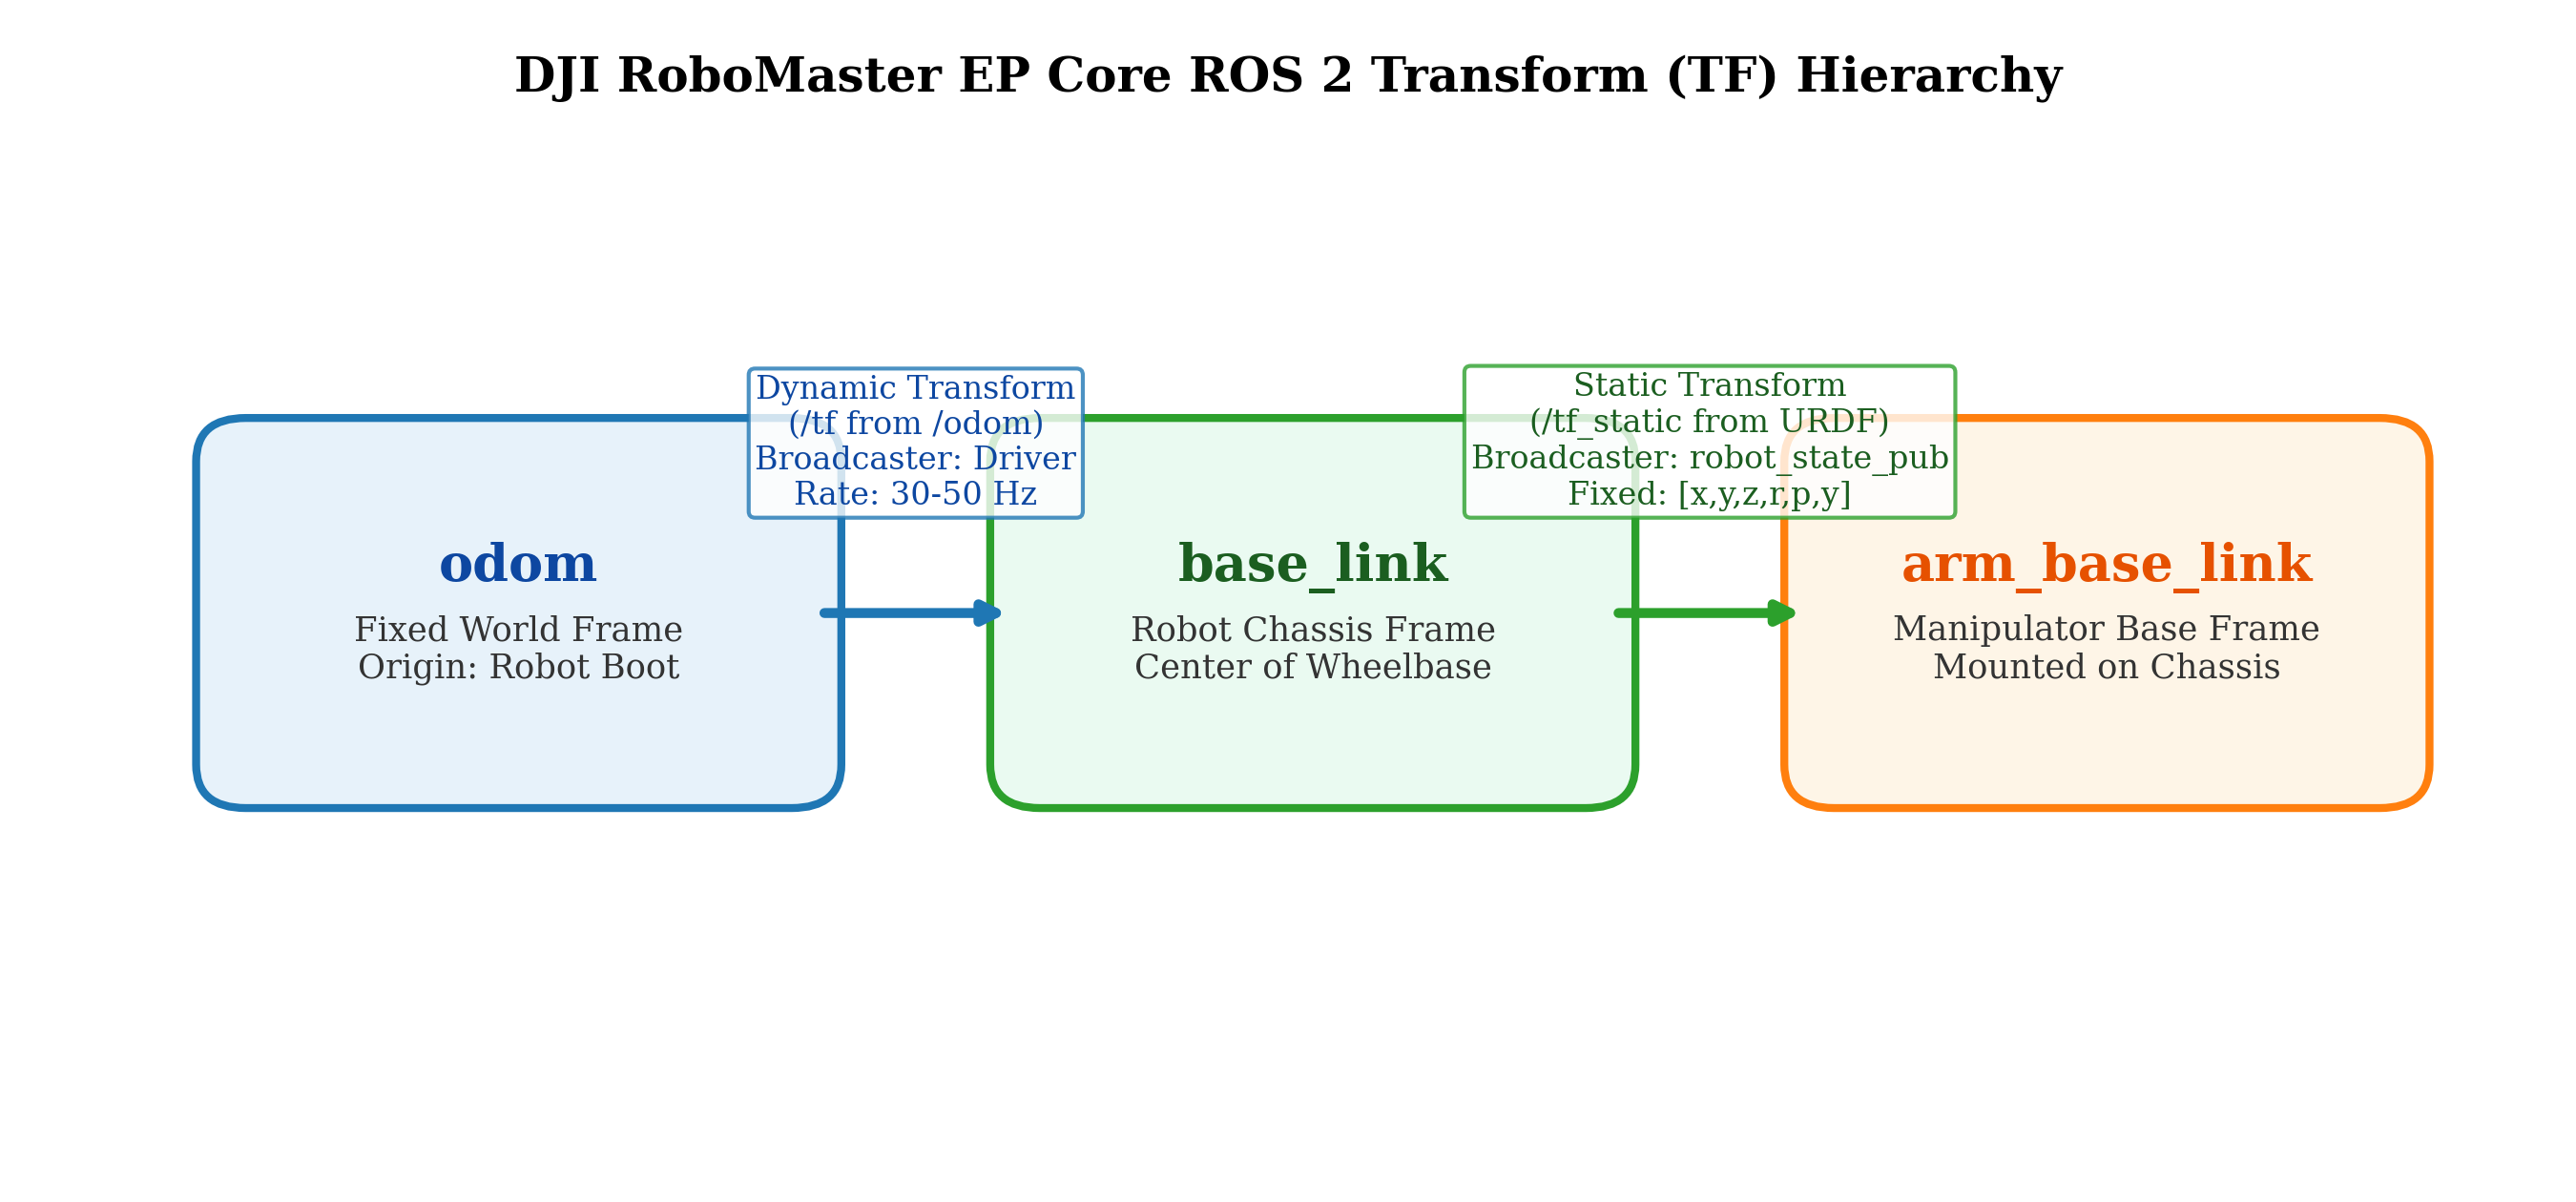
\includegraphics[height=2.2cm, width=0.80\linewidth, keepaspectratio]{fig_tf_tree.png}
\captionof{figure}{ROS 2 coordinate frame transform tree from \texttt{tf2\_tools view\_frames}.}
\label{fig:tf_tree}
\end{center}

\textbf{Transform Link Identification:}
\begin{enumerate}[noitemsep,topsep=1pt]
    \item \textbf{\texttt{odom} $\rightarrow$ \texttt{base\_link}:} Broadcast by \texttt{robomaster\_ros} driver node at 30~Hz from encoder and IMU dead-reckoning.
    \item \textbf{\texttt{base\_link} $\rightarrow$ \texttt{arm\_base\_link}:} Broadcast by \texttt{robot\_state\_publisher} at 50~Hz using static joint transforms from URDF.
\end{enumerate}

% =============================================================================
\section*{Deliverables Summary \& Video Demonstration Link}
% =============================================================================

\begin{center}
\small
\captionof{table}{Submission Deliverables Summary}
\label{tab:deliverables}
\vspace{0.1cm}
\begin{tabular}{>{\raggedright\arraybackslash}p{5.0cm} >{\raggedright\arraybackslash}p{10.0cm}}
\toprule
\textbf{Deliverable Item} & \textbf{File / Link Reference} \\
\midrule
\textbf{D1. Technical Report} & \texttt{report.pdf} (This document) \\
\textbf{D2. Workspace Code \& Repo} & \url{https://github.com/idiot28/sce672-assessment1} \\
                                    & \texttt{ep\_teleop\_sdk.py}, \texttt{rm\_setup.sh}, \\
                                    & \texttt{telemetry\_rndis\_30s.csv}, \texttt{telemetry\_ap\_30s.csv} \\
\textbf{D3. Video Demonstration} & \textit{[Insert your unlisted video URL here: e.g., https://youtu.be/...]} \\
\bottomrule
\end{tabular}
\end{center}

\textbf{Video Demonstration Artifact (D3):}
The video demonstration ($\le 45$ seconds) covers:
\begin{enumerate}[noitemsep,topsep=1pt]
    \item \textbf{Part A (0:00 -- 0:22):} Keyboard teleoperation with live terminal telemetry streaming using \texttt{ep\_teleop\_sdk.py}.
    \item \textbf{Part B (0:22 -- 0:45):} Driving the robot via ROS 2 keyboard teleoperation over direct Wi-Fi AP while echoing \texttt{/odom} in a secondary terminal.
\end{enumerate}

\end{document}
